\section{Multi-variate Polynomial Interpolation}

\begin{tabular}{ll}
  \parbox{6cm}{
    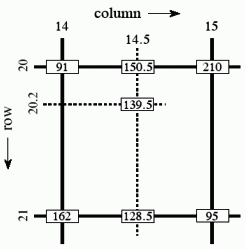
\includegraphics[width=6cm]{./bilder/bilineare_interpolation}
  }
  & \parbox{12.5cm} {
    \begin{itemize}
      \item The basis of polynomials can be calculated through the \emph{2-fold tensor product} $\Rightarrow$ Bilinear Interpolation \\
      $\{1,x,x^2\} \otimes \{1, y, y^2\} = \{1,x,y,x^2,y^2,xy, x^2y, xy^2, x^2y^2\}$; \\
      This way, the number of equations n can be calculated: \\$\mathbb R^n \otimes \mathbb R^k = \mathbb R^{nk}$
      \item Interpolate the desired order (linear, quadratic, \ldots) in the X-direction at position $y_0$: $p(x,y_0)$
      \item Interpolate the desired order (linear, quadratic, \ldots) in the X-direction at position $y_1$: $p(x,y_1)$
      \item Compute the tableau for divided differences (linear case here):\\
        \begin{tabular}{l|ll}
          $y$ & $z$\\
          \hline
          $y_0$ & $p(x,y_0) = a_{y0}$\\
          $y_1$ & $p(x,y_1)$ & $\frac{p(x,y_1) - p(x,y_0)}{y_1-y_0} = a_{y1}$
        \end{tabular}
      \item Formulate the polynomial:\\
        $p(x,y) = a_{y0} \pi_0(y) + a_{y1} \pi_1(y) + a_{y2} \pi_2(y)+\ldots$
      \item Expand the polynomial:\\
          $p(x,y) = a_{0,0} \pi_0(x)\pi_0(y) + a_{1,0} \pi_1(x)\pi_0(y) + a_{0,1} \pi_0(x)\pi_1(y) + a_{1,1} \pi_1(x)\pi_1(y)+\ldots$ 
    \end{itemize}
  }

\end{tabular}

\subsection{Example:}
Given points $(14,20),(14,21),(15,20)(15,21)$ with values $\{91/255, 162/255, 210/255, 95/255\}$. Linear interpolation is sought. 
This results in the following polynomial bases: $(\{1,x\}\times\{1,y\}=\{1,x,y,xy\})$\\
\begin{enumerate}
  \item Interpolation for $y=y_0=20$: $p(x,y_0)= p(x_0,y_0) \pi_0(x) + \frac{p(x_1,y_0)-p(x_0,y_0)}{x_1-x_0}\pi_1(x)=\frac{1}{255}\left(91 \cdot 1 + \frac{210-91}{15-14}\cdot(x-14)\right)$
  \item The same for $y=y_1=21$:  $p(x,y_1)=\frac{1}{255}\left(162 \cdot 1 + \frac{95-162}{15-14}\cdot(x-14)\right)$
  \item Then the final interpolation: $p(x,y)=p(x,y_0)\pi_0(y)+\frac{p(x,y_1)-p(x,y_0)}{y_1-y_0}\pi_1(y)$\\
  $=\frac 1{255} \left((91\cdot 1 +\frac{210-91}{15-14}\cdot 1)\cdot 1 + \frac{162\cdot 1 \frac{95-162}{15-14}\cdot (x-14)-91\cdot 1 + \frac{210-91}{15-14}\cdot(x-14)}{21-20}\cdot(y-20)\right)$
  $=-215.98 + 15.0549 x + 10.4902 y - 0.7294 x y$
\end{enumerate}

\todo[inline, color=red!50]{bi-cubic und multivariate}
